\section{Tagging}
The tagging part of the system is one of the primary pillars of the system. The implementation of the concept consists of multiple parts, such as the creation and maintenance of the tags, attaching tags to assets, searching for tags through assets, etc.
\par
Most of these parts have not been included in this section, because they are simply implemented and/or trivial. The parts chosen for this section are the connection between multiple tags, the connection to departments, and the attachment of tags to assets and the effects of this.

\subsection{Parent-child and department relation}
To better organize tags, as the user adds more to the system, each tag can belong to a department. This will decrease the number of tags being shown in the suggestions across the application and will make it easier to find the right tag. If a tag is universal, such as the user tag and a potential location tag, the department of the tag can be set to '\textit{All Departments}', in which case they will appear no matter the current department of the user.\\
The department separation of the tags improve the overall simplicity of the system, but a single department can still end up containing a huge amount of tags. To make it even easier to find the right tag, a hierarchical structure has been added through parent tags.
\par
Every tag belongs to a department, this is possibly \textit{All Departments}, but by the introduction of parent tags, they can also belong to another tag. This way, fields, color, and department of a tag can be inherited by other tags. This also makes it easier to create a number of tags with the same fields.\\
The hierarchic structure of the tags and their department only has three levels, as a parent tag cannot belong to a parent tag (see \autoref{fig:TagHierarchicStructureWithDepartment}).

\begin{figure}[H]
    \centering
    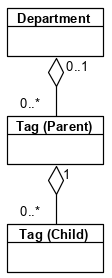
\includegraphics[width=0.2\textwidth]{figures/Implementation/TagHierarchicStructure.png}
    \caption{The hierarchic structure of the parent-child relation of tags}
    \label{fig:TagHierarchicStructureWithDepartment}
\end{figure}

The in this implementation, a tag is by default a parent tag without any children. A child tag is created by setting the parent tag of the tag to another tag. This means that a parent tag can have no children, but a child tag must have a parent, otherwise it will be a parent it self.\\
The connection between the parent and its child tags is an aggregation, but the children will inherit the fields, color, and department of the parent. The color can then be changed to something different, but the department is locked in place, as it will not be possible to access children belonging to another department than their parent.
\todo{Muligvis udvide med, hvordan parent tags og child tags bliver håndteret forskelligt i systemet? (Tagging an asset, searching assets through tags)}

\subsection{Asset-tag relation}
Attaching the tags to assets is the main purpose of the tags. When a tag is attached to an asset, the asset inherits the fields from the tag and an instance of the \textit{Asset-tag relation} class from the model component class diagram (see \autoref{fig:ModelComponentClassDiagram}) would be generated. This class, however, has not been implemented in the system, but exists in the database as a relation table between the asset and tag tables.
\par
A row in the relation table contains an id and the id of an asset and a tag. When fetching either assets or tags, the table can be used to get all the objects of the other class connected to wanted instance. This relation table also makes it possible to have multiple assets under one tag, without copying the tag to every asset and keeping the relation up to date, even if either the tag or the asset is updated.\\
This relational database also ensures that additional fields added to a tag can be added to the assets with the given tag, when they are opened for editing. The fields could be added automatically, but if the tag is attached to hundreds of assets, the value of the field would potentially have to be set for all these assets.
\par
The relational database also makes it possible to search for assets based on the tags attached to them. Below shows the method for retrieving all assets with at least one of the given tags attached (see ).

\begin{listing}[H]
\begin{minted}[frame=lines, framesep=3mm, baselinestretch=1, linenos, bgcolor=LightGray, escapeinside='', breaklines]{csharp}
    /// Searches the database for assets with one or more of the given tags
    /// </summary>
    /// <param name="tagIds">A list of IDs of the tags</param>
    /// <returns>An ObservableCollection of assets, containing the found assets (empty if no assets were found)</returns>
    public List<Asset> SearchByTags(List<int> tagIds)
    {
        var con = new MySqlHandler().GetConnection();
        List<Asset> assets = new List<Asset>();
    
        // Opening connection
        if (MySqlHandler.Open(ref con))
        {
            //"WHERE atr.tag_id IN (@ids) GROUP BY a.id";
            try
            {
                const string query = "SELECT a.* FROM assets AS a " + "INNER JOIN asset_tags AS atr ON (a.id = atr.asset_id) " + "WHERE atr.tag_id IN (@ids) AND deleted_at IS NULL GROUP BY a.id";
    
                using (var cmd = new MySqlCommand(query, con))
                {
                    cmd.Parameters.Add("@ids", MySqlDbType.String);
                    cmd.Parameters["@ids"].Value = string.Join(",", tagIds);
    
                    using (var reader = cmd.ExecuteReader())
                    {
                        while (reader.Read())
                        {
                            assets.Add(DataMapper(reader));
                        }
                        reader.Close();
                    }
                }
            }
            catch (MySqlException e)
            {
                Console.WriteLine(e);
            }
            finally
            {
                con.Close();
            }
        }
    
        return assets;
    }
\end{minted}
\captionof{listing}{TagRepository SearchByTags method}
\label{code:TagRepositorySearchByTags}
\end{listing}

The method takes in a list of tag IDs